\section{Argument Schemes for Goal Modeling}
\label{sect:gmas}

\begin{table*}[h]
\centering
\begin{tabularx}{\textwidth}{|l|l|l|X|l|l|}
\hline
\multicolumn{2}{|c|}{\textbf{Argument scheme}} & \multicolumn{2}{c|}{\textbf{Critical Questions}} & \textbf{Effect}\\
\hline
AS0 & Actor $a$ is relevant & CQ0 &Is the actor relevant? & DISABLE\\
\hline
AS1 & Actor $a$ has resource $R$ & CQ1 &Is the resource available? & DISABLE\\
\hline
AS2 & Actor $a$ can perform task $T$ & CQ2 &Is the task possible? & DISABLE\\
\hline
AS3 & Actor $a$ has goal $G$ & CQ3 & Can the desired goal be realized? & DISABLE\\
\hline
AS4 & Actor $a$ has softgoal $S$ & CQ4 & Is the softgoal a legitimate softgoal?& DISABLE\\
\hline
\hline
AS5 & Goal $G$ decomposes into tasks $T_1,\ldots,T_n$ & CQ5a & Does the goal decompose into the tasks?& DISABLE\\
& & CQ5b & Does the goal decompose into any other tasks?& REPLACE\\
\hline
AS6 & Task $T$ contributes to softgoal $S$& CQ6a & Does the task contribute to the softgoal?& DISABLE\\
&& CQ6b & Are there alternative ways of contributing to the same softgoal?& INTRO \\
&& CQ6c & Does the task have a side effect which contribute negatively to some other softgoal?& INTRO\\
&& CQ6d & Does the task contribute to some other softgoal?& INTRO\\
\hline
AS7 & Goal $G$ contributes to softgoal $S$ & CQ7a & Does the goal contribute to the softgoal?& DISABLE\\
&& CQ7b & Does the goal contribute to some other softgoal?& INTRO\\
\hline
AS8 & Resource $R$ contributes to task $T$ & CQ8 & Is the resource required in order to perform the task?& DISABLE\\
\hline
AS9 & Actor $a$ depends on actor $b$ & CQ9 & Does the actor depend on any actors?& INTRO\\
\hline
AS10 & Task $T_1$ decomposes into tasks $T_2,\ldots,T_n$ & CQ10a & Does the task decompose into other tasks?& REPLACE\\
 &  & CQ10b & Is the decomposition type correct? (AND/OR/XOR)& REPLACE\\
\hline
AS11 & Task $T$ contributes negatively to softgoal $S$& CQ11 & Does the task contribute negatively to the softgoal?& DISABLE\\
\hline
\hline
AS12 & Element $IE$ is relevant & CQ12 & Is the element relevant/useful? & DISABLE\\
\hline
AS13 & Element $IE$ has name $n$ & CQ13 & Is the name clear/unambiguous? & REPLACE\\
\hline
\hline
- & - & Att & Generic counterargument & ATTACK\\
\hline
\end{tabularx}
\caption{List of argument schemes (AS0-AS13, left column), critical questions (CQ0-CQ12, middle column), and the effect of answering them (right column).}
\label{table:argument-schemes}
\end{table*}

In the previous section we provided an overview of RationalGRL. In the example of the methodology, we discussed various argument schemes and critical questions. In this section, we discuss our argument schemes and critical questions in more detail. It is important to note that the list of argument schemes we obtain in this section is not exhaustive. It is an initial list that we obtained by annotating transcripts, but our framework is fully extensible, meaning that new argument schemes and critical questions can be added depending on the problem domain.

The list of argument schemes and critical questions that we obtained from our analysis is shown in Table~\ref{table:argument-schemes}. The first four argument schemes (AS0-AS4) are arguments for an element of a goal model, the next seven (AS5-AS11) are about relationships, the next two (AS12-AS13) are about intentional elements in general, and the last is (Att) is a generic counterargument for any type of argument that has been put forward.

As we already discussed in the methodology, we found that answering critical questions can have varying effects on the model, and for each critical question, the right column in Table~\ref{table:argument-schemes} shows the effect of answering the critical questions affirmatively. Answering a critical questions can create an argument disabling the corresponding GRL element of the attacked argument scheme (\textsf{DISABLE}); it can create an argument introducing a new GRL element (\textsf{INTRO}); it can replace the GRL element corresponding to the original argument (\textsf{REPLACE}), or it can simply attack an argument directly (\textsf{ATTACK}).

In the first subsection of this section, we provide details of the transcript annotation process with concrete examples (see Appendix~\ref{sect:transcripts:excerpts} for transcript excerpts), after which we analyze our results in the second subsection.

\subsection{Details experiment}

The transcripts we used are created as part of two master theses on improving design reasoning~\cite{masterthesis1,masterthesis2}.

\paragraph{Subjects} The subjects for the case study are three teams of Master students from the University of Utrecht, following a Software Architecture course. Two teams consist of three students, and one team consists of two students.

\paragraph{Experimental Setup} The assignment used for the experiments is to design a traffic simulator. Participants were asked to use a think-aloud method during the design session. The assignment was slightly adjusted to include several viewpoints as end products in order to conform to the course material~\cite{Bass:2012:SAP:2392670}. The full problem descriptions can be found in Appendix~\ref{sect:designprompt}. All groups were instructed to apply the \emph{functional architecture method}, focusing on developing the \emph{context}, the \emph{functional}, and the \emph{informational} viewpoints of the traffic simulator software. The students had two hours for the tasks, and the transcripts document the entire discussion. The details of the transcripts are shown in Table~\ref{table:transcripts:info}.

\begin{table}[ht]
\centering
\begin{tabular}{|l|l|l|l|}
\hline
& transcript $t_1$ & transcript $t_2$ & transcript $t_3$\\
\hline
participants & 2 & 3 & 3\\
\hline
duration & 1h34m52s & 1h13m39s & 1h17m20s\\
\hline
\end{tabular}
\caption{Number of participants and duration of the transcripts.}
\label{table:transcripts:info}
\end{table}

\paragraph{Annotation Method} 

We started with an initial list of 8 argument schemes and 18 critical questions that we derived from PRAS (AS1-AS4, AS6-AS9 of Table~\ref{table:argument-schemes}). We annotated transcripts with the arguments and critical questions from this list. If we found arguments or critical questions that did not appear in the original list, we added them and counted them as well. Argument schemes that did not appear were removed from the list, but critical questions were not removed (see discussion in Section~\ref{sect:gmas:transcripts:analysis}). Most of the occurrences were not literally found back, but had to be inferred from the context. This can be seen in the various examples we will discuss.

It is generally known in the argumentation literature that it can be very difficult to identify arguments in natural language texts~\cite{walton-etal2004}. Arguments are often imprecise, lack conclusion, and may be supported by non verbal communication that is not captured in the transcripts. However, there is hardly any research on on argument extraction in the requirement engineering domains, so despite this potential weakness in our approach, we believe it nevertheless is at least useful as something that others can build further on (see Section~\ref{sect:goalmodeling:openissues}).

\paragraph{Results}

\begin{figure*}[h]
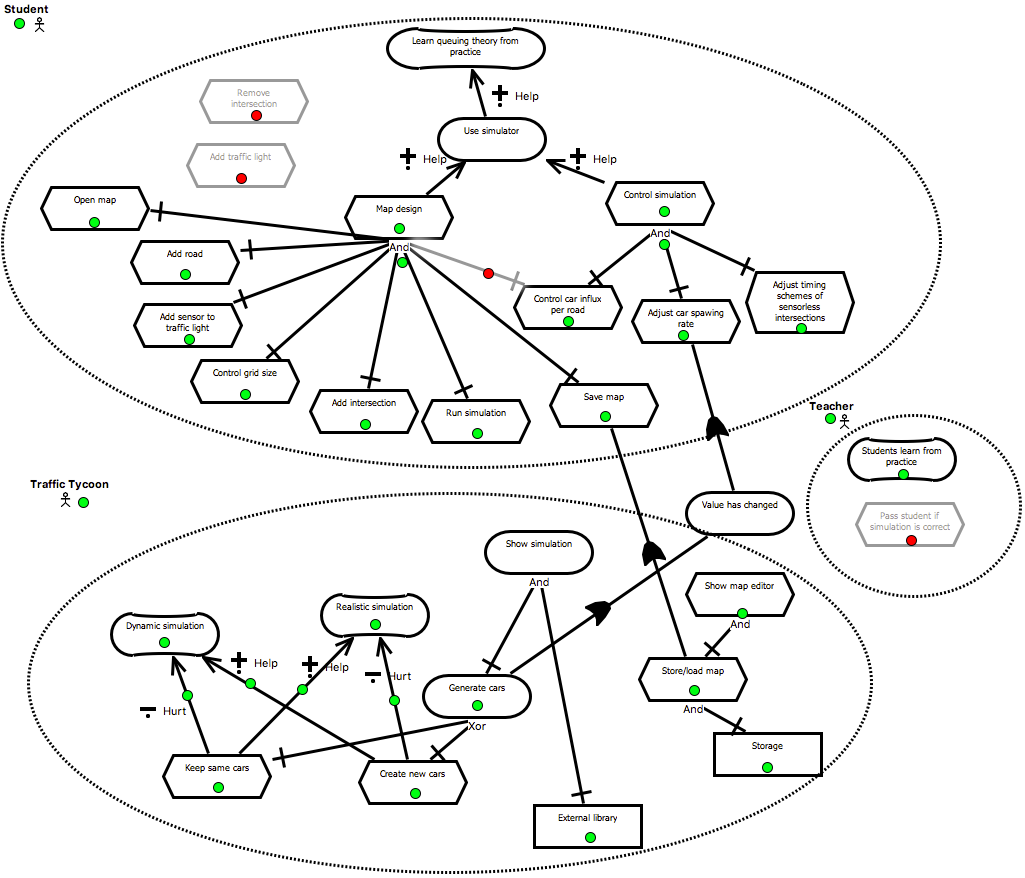
\includegraphics[width=\textwidth]{img/transcript_grl}
\caption{The GRL model manually constructed from transcript $t_1$. Green dots indicate accepted underlying arguments, red dots indicate rejected underlying arguments. Elements and relationships with no dot have been inferred by us.}
\label{fig:transcripts:grl}
\end{figure*}

All original transcripts, annotations, and models are available on the following website \todo{Marc}{Marc}{Change URL and put everything together with the tool}:
\begin{quote} \url{http://www.github.com/marcvanzee/RationalArchitecture}
\end{quote}
We also provide excerpts of the annotation in Appendix~\ref{sect:transcripts:excerpts}, and most of the examples we use in this article come from the transcripts.

We found a total of 159 instantiations of the argument schemes AS0-AS11 in the transcripts. The most used argument scheme was AS2: ``Actor $A$ has task $T$'', but each argument scheme has been found back in the transcripts at least twice (Table~\ref{table:transcripts:results:argumentschemes}). A large portion (about 60\%) of the argument schemes we found involved discussions around tasks of the information system (AS2, AS10).

We annotated 41 applications of critical questions. Many critical questions (about 55\%) involved clarifying the name of an element, or discussing the relevance of it (CQ12, CQ13).

\begin{table}[ht]
\centering
\begin{tabularx}{0.5\textwidth}{|l|X|l|l|l|>{\bfseries}l|}
\hline
\multicolumn{2}{|c|}{\textbf{Scheme/Question}} & $t_1$ & $t_2$ & $t_3$ & \textbf{total}\\
\hline 
AS0 & Actor & 2 & 2 & 5 & 9\\
\hline
AS1 & Resource & 2 & 4 & 5 & 11\\
\hline
AS2 & Task/action & 20 & 21 & 17 & 58\\
\hline
AS3 & Goal & 0 & 2 & 2 & 4\\
\hline
AS4 & Softgoal & 3 & 4 & 2 & 9\\
\hline
AS5 & Goal decomposes into tasks & 4 &0& 4 & 8\\
\hline
AS6 & Task contributes to softgoal & 6 & 2 &0& 8\\
\hline
AS7 & Goal contributes to softgoal &0& 1 & 1 & 2\\
\hline
AS8 & Resource contributes to task & 0 & 4 & 3 & 7\\
\hline
AS9 & Actor depends on actor &0& 1 & 3 & 4\\
\hline
AS10 & Task decomposes into tasks & 11 &14 &11 &36\\ 
\hline
AS11 & Task contributes negatively to softgoal & 2 & 1 & 0 & 3\\
\hline
\hline
CQ2 & Task is possible? & 2 & 2 & 1 & 5\\
\hline		
CQ5a & Does the goal decompose into the tasks? & 0 & 1 & 0 & 1\\
\hline
CQ5b & Goes decomposes into other tasks? & 1 & 0 & 0 & 1\\
\hline
CQ6b & Task has negative side effects? & 2 & 0 & 0 & 2\\
\hline
CQ10a & Task decompose into other tasks? & 1 &2 &0&3\\
\hline
CQ10b & Decomposition type correct? &1 &0& 1 &2\\
\hline
\hline
CQ12 & Is the element relevant/useful? & 2 & 3 & 2 &7\\
\hline
CQ13 & Is the name clear/unambiguous? &3 &10 & 3 & 16\\
\hline
\hline
- & Generic counterargument & 0& 2 & 2 & 4\\
\hline
\hline
\multicolumn{2}{|c|}{\textbf{TOTAL}}&69&80&69&222\\
\hline
\end{tabularx}
\caption{Number of occurrences of AS0-AS9, CQ0-CQ12 in the transcripts. Critical questions not appearing in this table were not found back in the transcripts.}
\label{table:transcripts:results:argumentschemes}
\end{table}

For each transcript, we manually created a GRL model from the argument schemes and critical questions we found in them, in order to verify whether the arguments put forward by the participants were sufficiently informative. An example of such a model is shown in Figure~\ref{fig:transcripts:grl}. We added green and red dots to various elements and relationships in the figure. A green dot indicates there is an underlying argument for the element that is accepted, while a red dot indicates a rejected underlying argument. Note that if the underlying argument is rejected, the corresponding GRL element has been disabled. Some elements do not have a corresponding green or red dot. In that case, we have inferred the elements from the discussion, but we could not explicitly find back arguments for it.

We found that answering a critical questions can have four different effects on the original argument and the corresponding GRL element:
\begin{itemize}
\item \textsf{INTRO}: Introduce a new goal element or relationship with a corresponding argument. This operation does not attack the original argument of the critical question, but rather creates a new argument. For instance, suppose argument scheme AS5 is instantiated as follows:: ``Goal \texttt{Generate cars} OR-decomposes into tasks \texttt{Keep same cars} and \texttt{Create new cars}''. Suppose now the critical question CQ5b: ``Does the goal \texttt{Agreeable meeting dates} decompose into other tasks?'' is answered with ``yes, namely \texttt{Choose randomly}''. This results in a new instantiation of AS5, namely: ``Goal \texttt{Generate cars} OR-decomposes into tasks \texttt{Keep same cars}, \texttt{Create new cars}, and \texttt{Choose randomly}. As a result, the goal model will contain the corresponding task \texttt{Choose randomly}, as well as an OR-decomposition relation from the goal \texttt{Generate cars} to that task.
\item \textsf{DISABLE:} Disable the element or relationship of the argument scheme to which the critical questions pertains. This operation does not create a new argument, but only disables (i.e., attacks) the original one. For instance, suppose argument scheme AS0 is instantiated with: ``Actor \texttt{Teacher} is relevant''. This argument can be attack with critical question CQ0: ``Actor \texttt{Teacher} is not relevant''. As a result, the argument for the actor is attack, and actor \texttt{Teacher} is disabled in the goal model.
\item \textsf{REPLACE:} Replace the element of the argument scheme with a new element. This operation both introduces a new argument and attacks the original one. For instance, suppose argument scheme AS2 is instantiated with: ``Actor \texttt{Student} can perform task \texttt{Choose a pattern preference}. This argument can be attacked with critical question CQ13: ``The task \texttt{Choose a pattern preference} is unclear, it should be \texttt{Choose a road pattern}''. This results in replacing the original argument with the new argument ``Actor \texttt{Student} can perform task \texttt{Choose a road pattern}. In the goal model, the description of the task should change accordingly.
\item \textsf{ATTACK:} Attack any argument with an argument that cannot be classified as a critical question. For instance, suppose argument scheme AS0 is instantiated with ``Actor \texttt{Teacher} is relevant''. Suppose this argument is attacked with critical question CQ0: ``Actor \texttt{Teacher} is not relevant'', because she does not create the system. However, this critical question may in turn be attacked again, if new evidence comes up. For instance, it may turn out that the teacher will work on developing the application herself. In this case, the generic counter argument ``Actor \texttt{Teacher} is relevant, because does develop for the application'' attack the argument ``Actor \texttt{Teacher} is not relevant''. As a result, the original argument ``Actor \texttt{Teacher} is relevant'' is accepted again, and as a result is shown in the goal model.
\end{itemize}

In Section~\ref{sect:examples} we provide examples we found in the transcripts for all of these four effects.

\subsection{Analysis}
\label{sect:gmas:transcripts:analysis}

\paragraph{Analysis of the Argument Schemes}
Recall that our initial list of argument schemes consists of AS1-AS4, AS6-AS9 (Table~\ref{table:argument-schemes}). Therefore, the difference between the initial list of argument schemes and those found back in the transcripts is quite small. We found it surprising that we were able to find back all the schemes in the transcript at least twice, even more since the topic of discussion was not goal models, but more generally the architecture of an information system. This gives us an indication that it is possible to capture (parts of the) arguments used in those type of discussions using argument schemes.

We observed that our initial list is rather limited, which is a consequence of the fact that it is derived from PRAS. Since PRAS only considers very specific types of relationships, we are not able to capture many other relationships existing in GRL. GRL has four types of intentional elements (softgoal, goal, task, resource) and four types of relationships (positive contribution, negative contribution\footnote{In fact, a contribution can be any integer in the domain [-100,100], but for the sake of simplicity we only consider two kinds of contributions here.}, dependency, decomposition), allowing theoretically $4^3=64$ different types of argument schemes, of which we currently only consider 11. Our analysis however shows that many of these schemes are not often used, and thus, gives us some confidence in the resulting list. However, additional argument schemes and critical questions can be added freely to our framework, and our list is not meant to be exhaustive.

\paragraph{Analysis of the Critical Questions} The difference between the initial list of critical questions and those we found back in the transcripts is much larger than for the critical questions. %SG: I don't get this sentence. Also, the ones below. 
We found few of the critical questions we initially proposed. However, this does not mean that they were not implicitly used in the minds of the participants. If a participants for instance forms an argument for a contribution from a task to a softgoal, it may very well be that she was asking herself the question ``Does the task contribute to some other softgoal?''. However, many of these critical questions are not mentioned explicitly. If we assume this explanation is at least partially correct, then this would mean that critical questions may still play a role when formalizing the discussions leading up to a goal model, and it would be limiting to leave them out of our framework. In the context of tool support, we believe that having these critical questions available may stimulate discussions.